% Generated from completed canonical matrices; no controller training.
\section{Resultados da avaliação unificada}
\label{sec:resultados_unificados}
\begin{table}[htbp]\centering\small
\caption{Bahia: resultados por caso série--origem. Custo: 290 casos; atendimento: 283 casos definidos. Custo em unidades de cenário.}
\label{tab:unificado_ba}
\begin{tabular}{@{}p{4.4cm}rrrr@{}}\toprule
Implementação & Custo médio & Atendimento & Viáveis & Trocas\\\midrule
Referência global & 161,31 & 73,62\% & 164 & 0\\
PSE por perfil & 164,41 & 77,51\% & 183 & 80\\
PSE por classe (XGBoost) & 166,57 & 70,04\% & 155 & 206\\
Classe: floresta de controle & 155,79 & 68,16\% & 154 & 143\\
Consequências & 159,05 & 72,77\% & 165 & 106\\
Consequências sem perfil & 161,65 & 74,07\% & 170 & 90\\
Consequências com recuo & 161,31 & 73,62\% & 164 & 0\\
\bottomrule\end{tabular}
\par\footnotesize Trocas indicam política diferente da referência global; viáveis têm atendimento $\geq0{,}70$.
\end{table}
\begin{table}[htbp]\centering\small
\caption{M5: resultados por caso série--origem. Custo: 5326 casos; atendimento: 5138 casos definidos. Custo em unidades de cenário.}
\label{tab:unificado_m5}
\begin{tabular}{@{}p{4.4cm}rrrr@{}}\toprule
Implementação & Custo médio & Atendimento & Viáveis & Trocas\\\midrule
Referência global & 779,46 & 68,27\% & 2448 & 0\\
PSE por perfil & 780,80 & 68,49\% & 2471 & 411\\
PSE por classe (XGBoost) & 811,31 & 65,37\% & 2255 & 4259\\
Classe: floresta de controle & 812,42 & 63,99\% & 2177 & 4299\\
Consequências & 760,45 & 68,08\% & 2456 & 3629\\
Consequências sem perfil & 761,77 & 67,92\% & 2440 & 3655\\
Consequências com recuo & 764,20 & 68,59\% & 2472 & 679\\
\bottomrule\end{tabular}
\par\footnotesize Trocas indicam política diferente da referência global; viáveis têm atendimento $\geq0{,}70$.
\end{table}
\begin{figure}[htbp]\centering
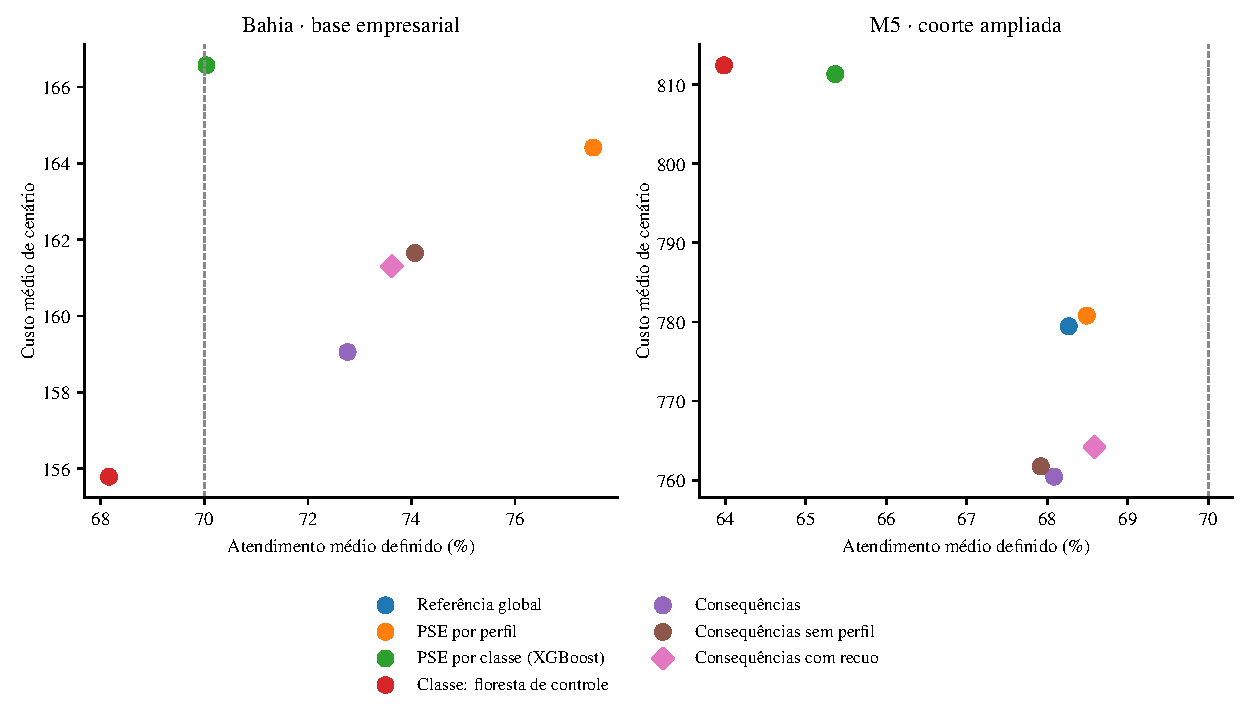
\includegraphics[width=\linewidth]{figures/aipe_unificado_custo_servico_20261017.pdf}
\caption{Custo e atendimento nas duas aplicações. As médias não mostram a distribuição individual nem constituem fronteira de dominância por série.}\label{fig:unificado_custo_servico}
\end{figure}
\begin{figure}[htbp]\centering
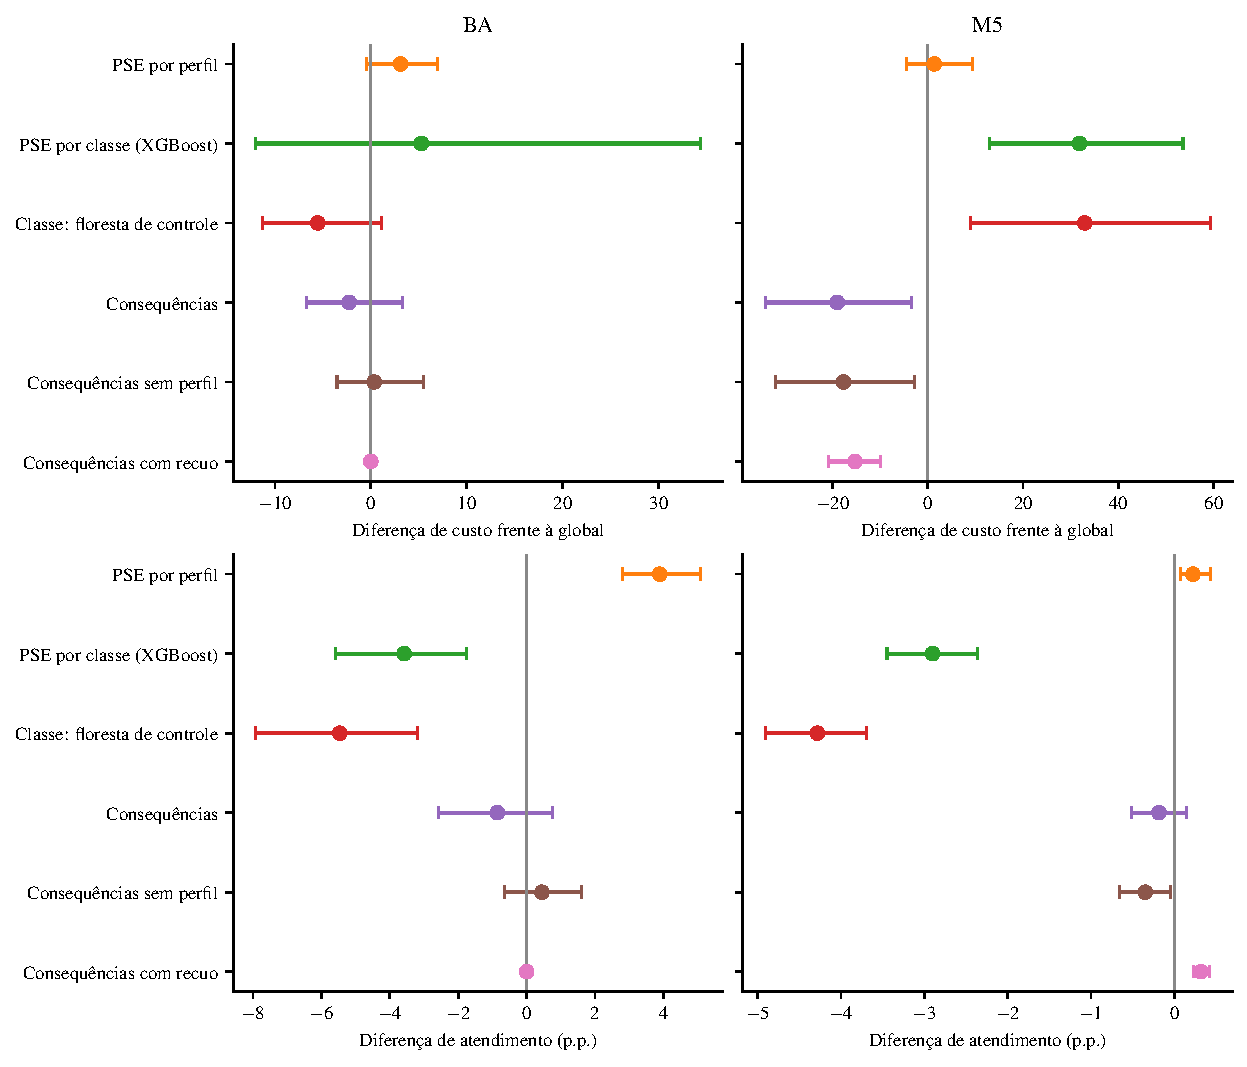
\includegraphics[width=\linewidth]{figures/aipe_unificado_diferencas_20261017.pdf}
\caption{Diferenças pareadas frente à referência global. Intervalos condicionais por loja, preservando produtos e origens; dez lojas limitam a precisão no M5.}\label{fig:unificado_diferencas}
\end{figure}
\begin{figure}[htbp]\centering
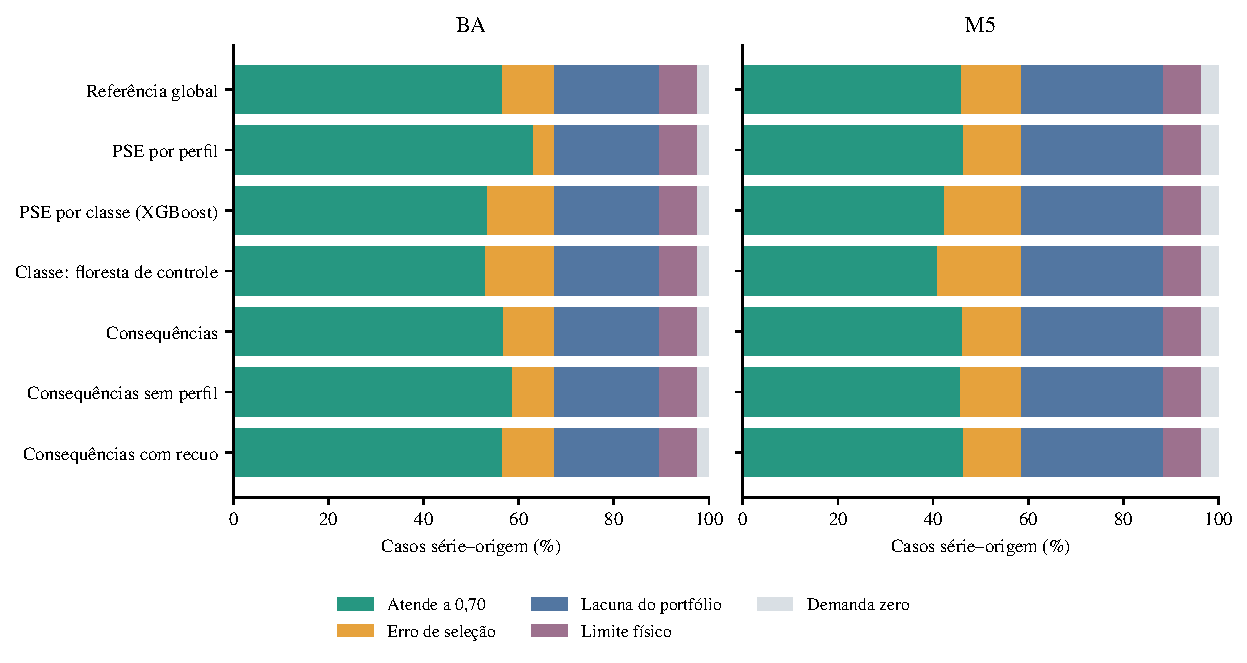
\includegraphics[width=\linewidth]{figures/aipe_unificado_falhas_20261017.pdf}
\caption{Diagnóstico retrospectivo dos casos. A classificação distingue falha de seleção, cobertura do portfólio e restrição física inicial; demanda zero mantém atendimento indefinido.}\label{fig:unificado_falhas}
\end{figure}
\begin{figure}[htbp]\centering
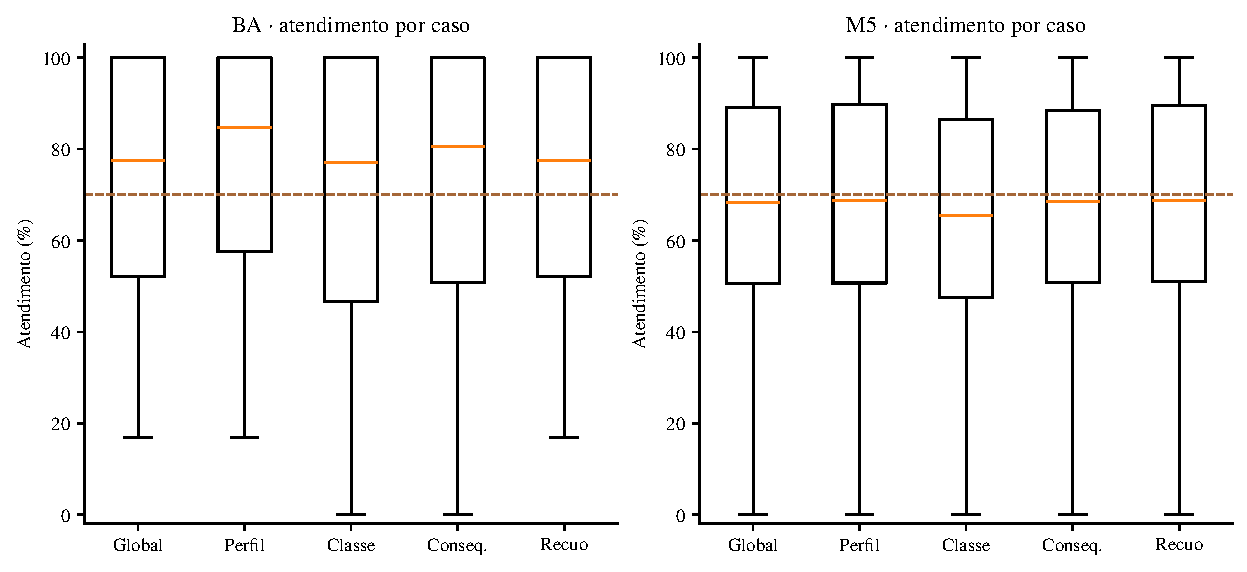
\includegraphics[width=\linewidth]{figures/aipe_unificado_distribuicao_20261017.pdf}
\caption{Distribuição do atendimento nos casos com demanda positiva; linha horizontal indica 70\%. Extremos são omitidos da exibição dos boxplots, mas permanecem nos cálculos.}\label{fig:unificado_distribuicao}
\end{figure}
